\documentclass[12pt]{article}

\usepackage[a4paper,margin=0.5in]{geometry}
\usepackage{graphicx}
\usepackage{float}
\usepackage{amssymb}

\begin{document}

\begin{figure}[H]
    \centering
    
\includegraphics[width=1.0\textwidth]{test.png}
\end{figure}

The figure above provides an overview of simulations with small $R_{\rm cut}$ values. For $R_{\rm cut} \gtrsim 0.1\,\mathrm{kpc}$, the system evolves very similarly to the reference (vanilla SWIFT) run. However, as $R_{\rm cut}$ approaches the softening length value, the cusp-to-core transition does not extend to large timesteps.\\

This behaviour is clearly illustrated in the following figures: while the simulation with $R_{\rm cut}=5\,\mathrm{kpc}$ exhibits continued core growth up to $100\,\mathrm{Gyr}$, progressively smaller values of $R_{\rm cut}$ lead to increasingly limited core evolution, eventually resulting in a density profile that does not decrease.

\begin{figure}[H]
    \centering
    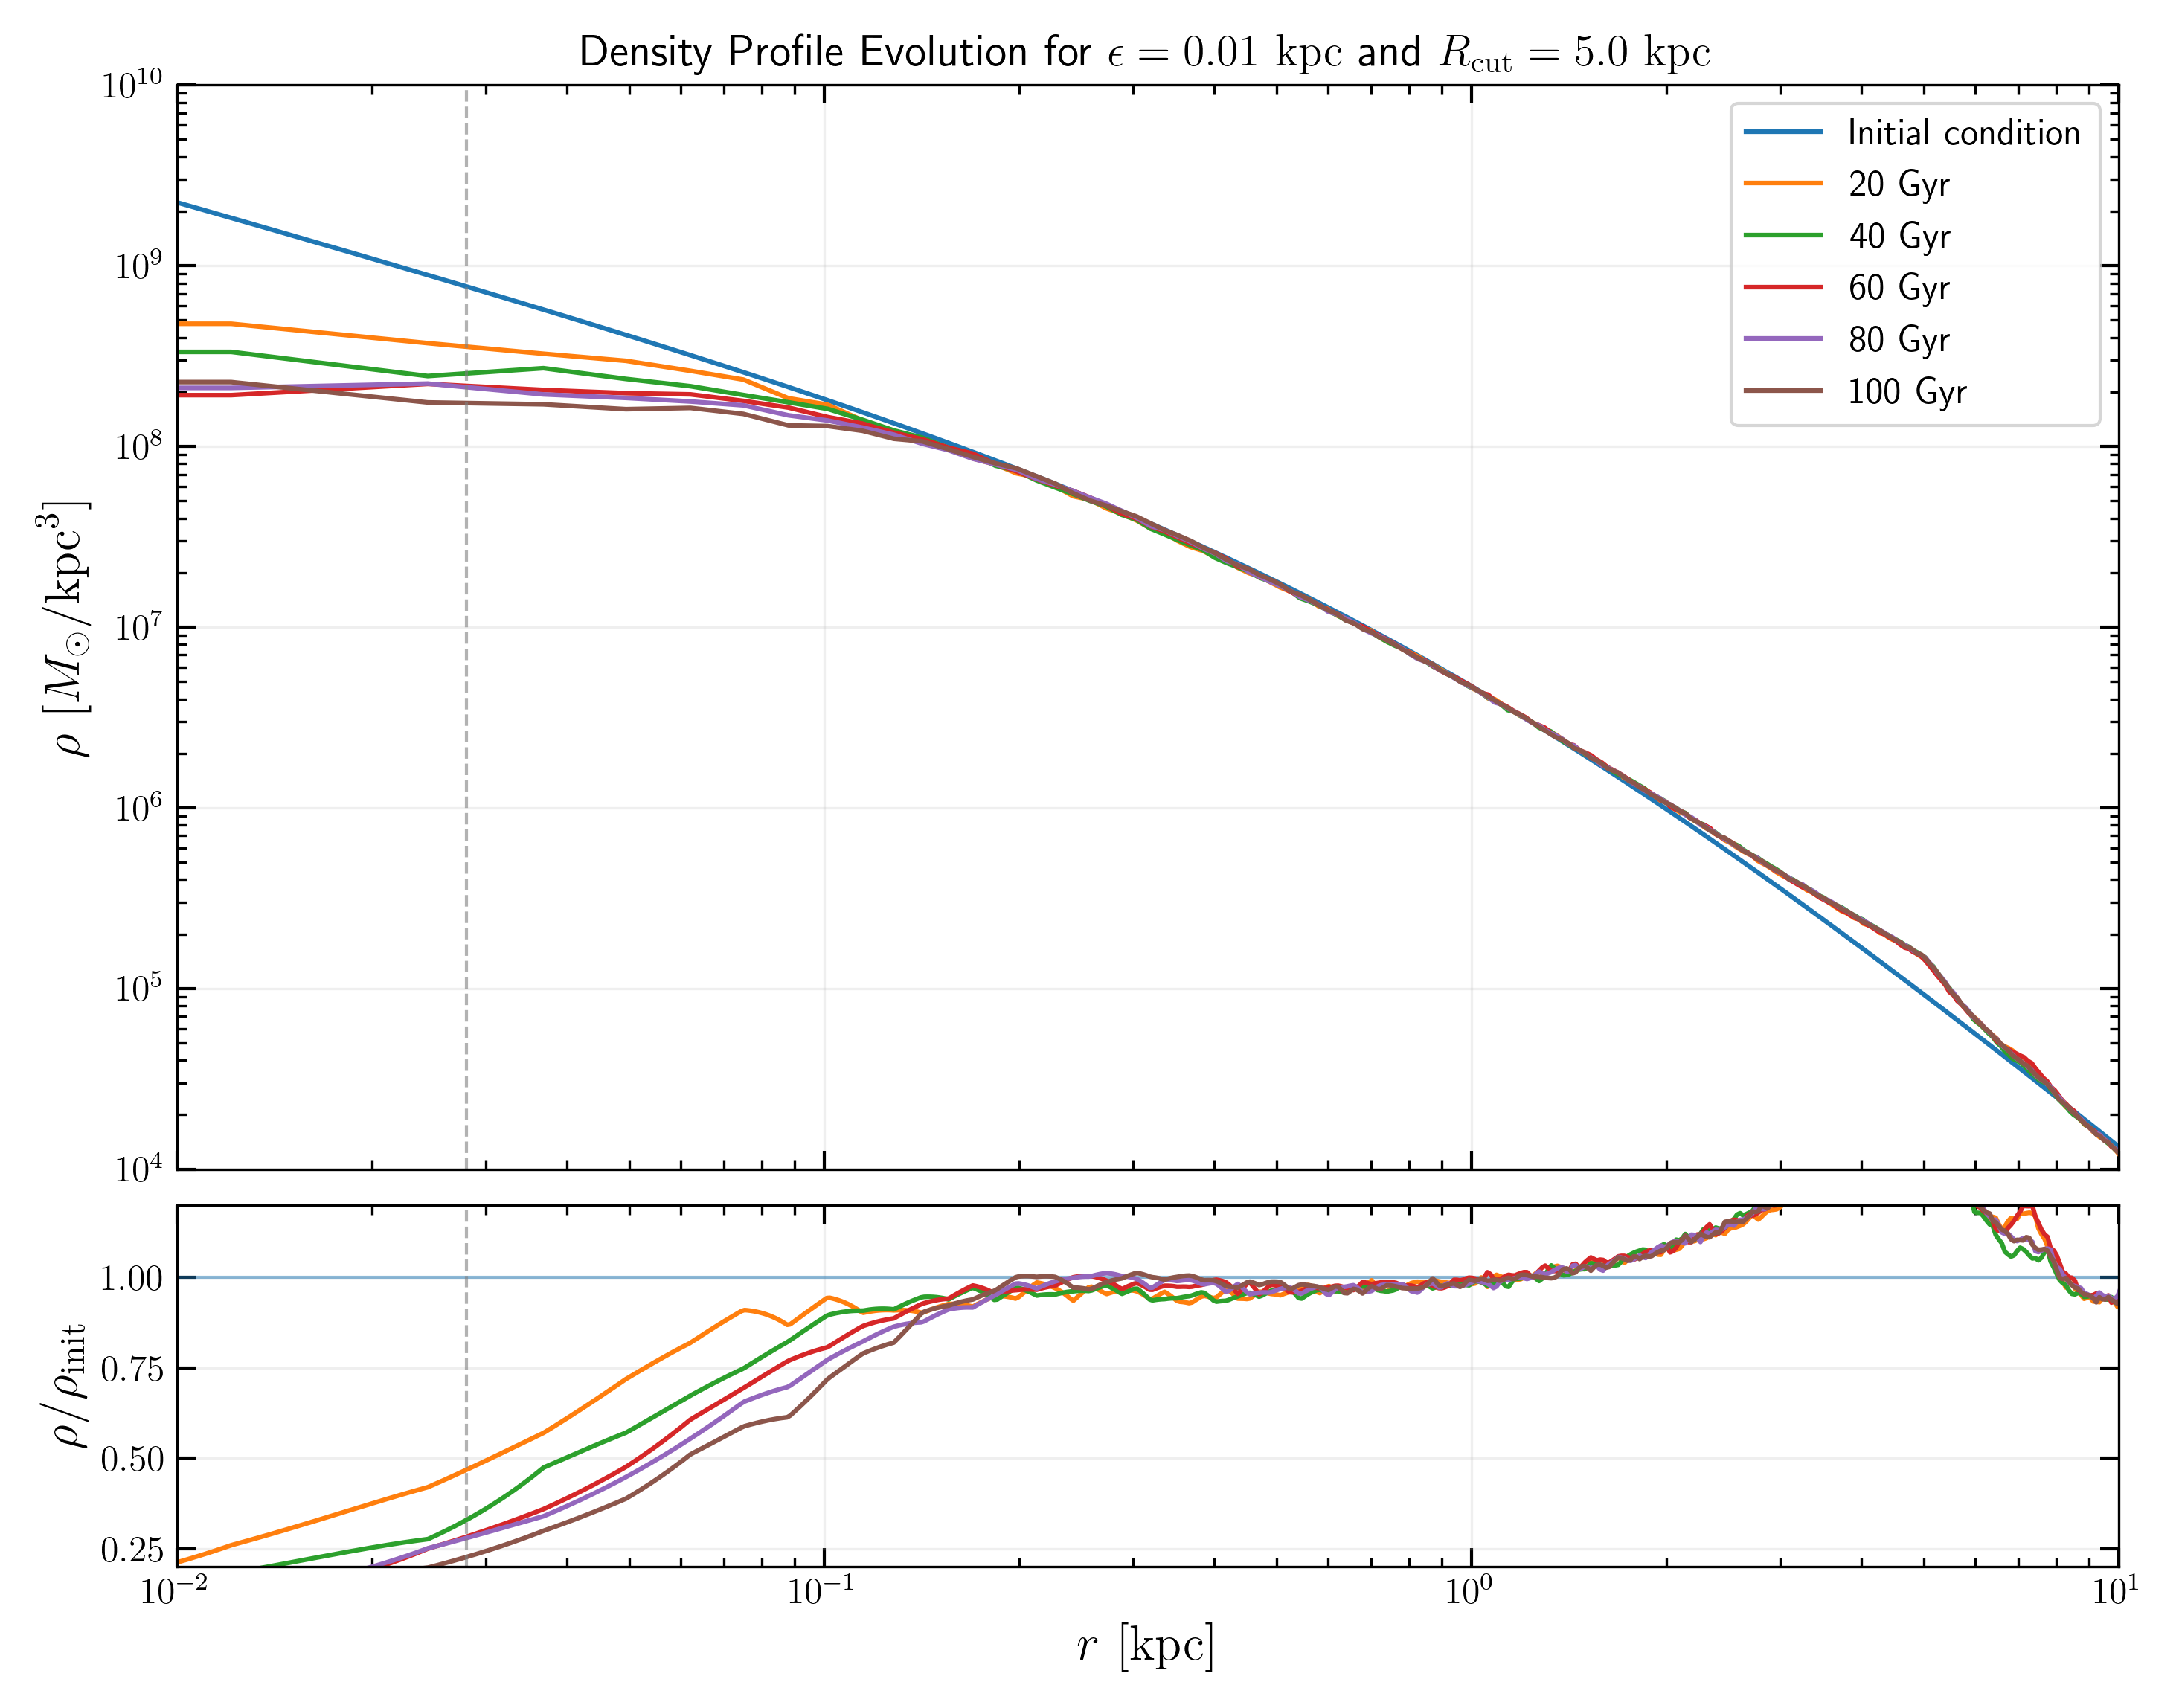
\includegraphics[width=0.9\textwidth]{5.png}
\end{figure}

\begin{figure}[H]
    \centering
    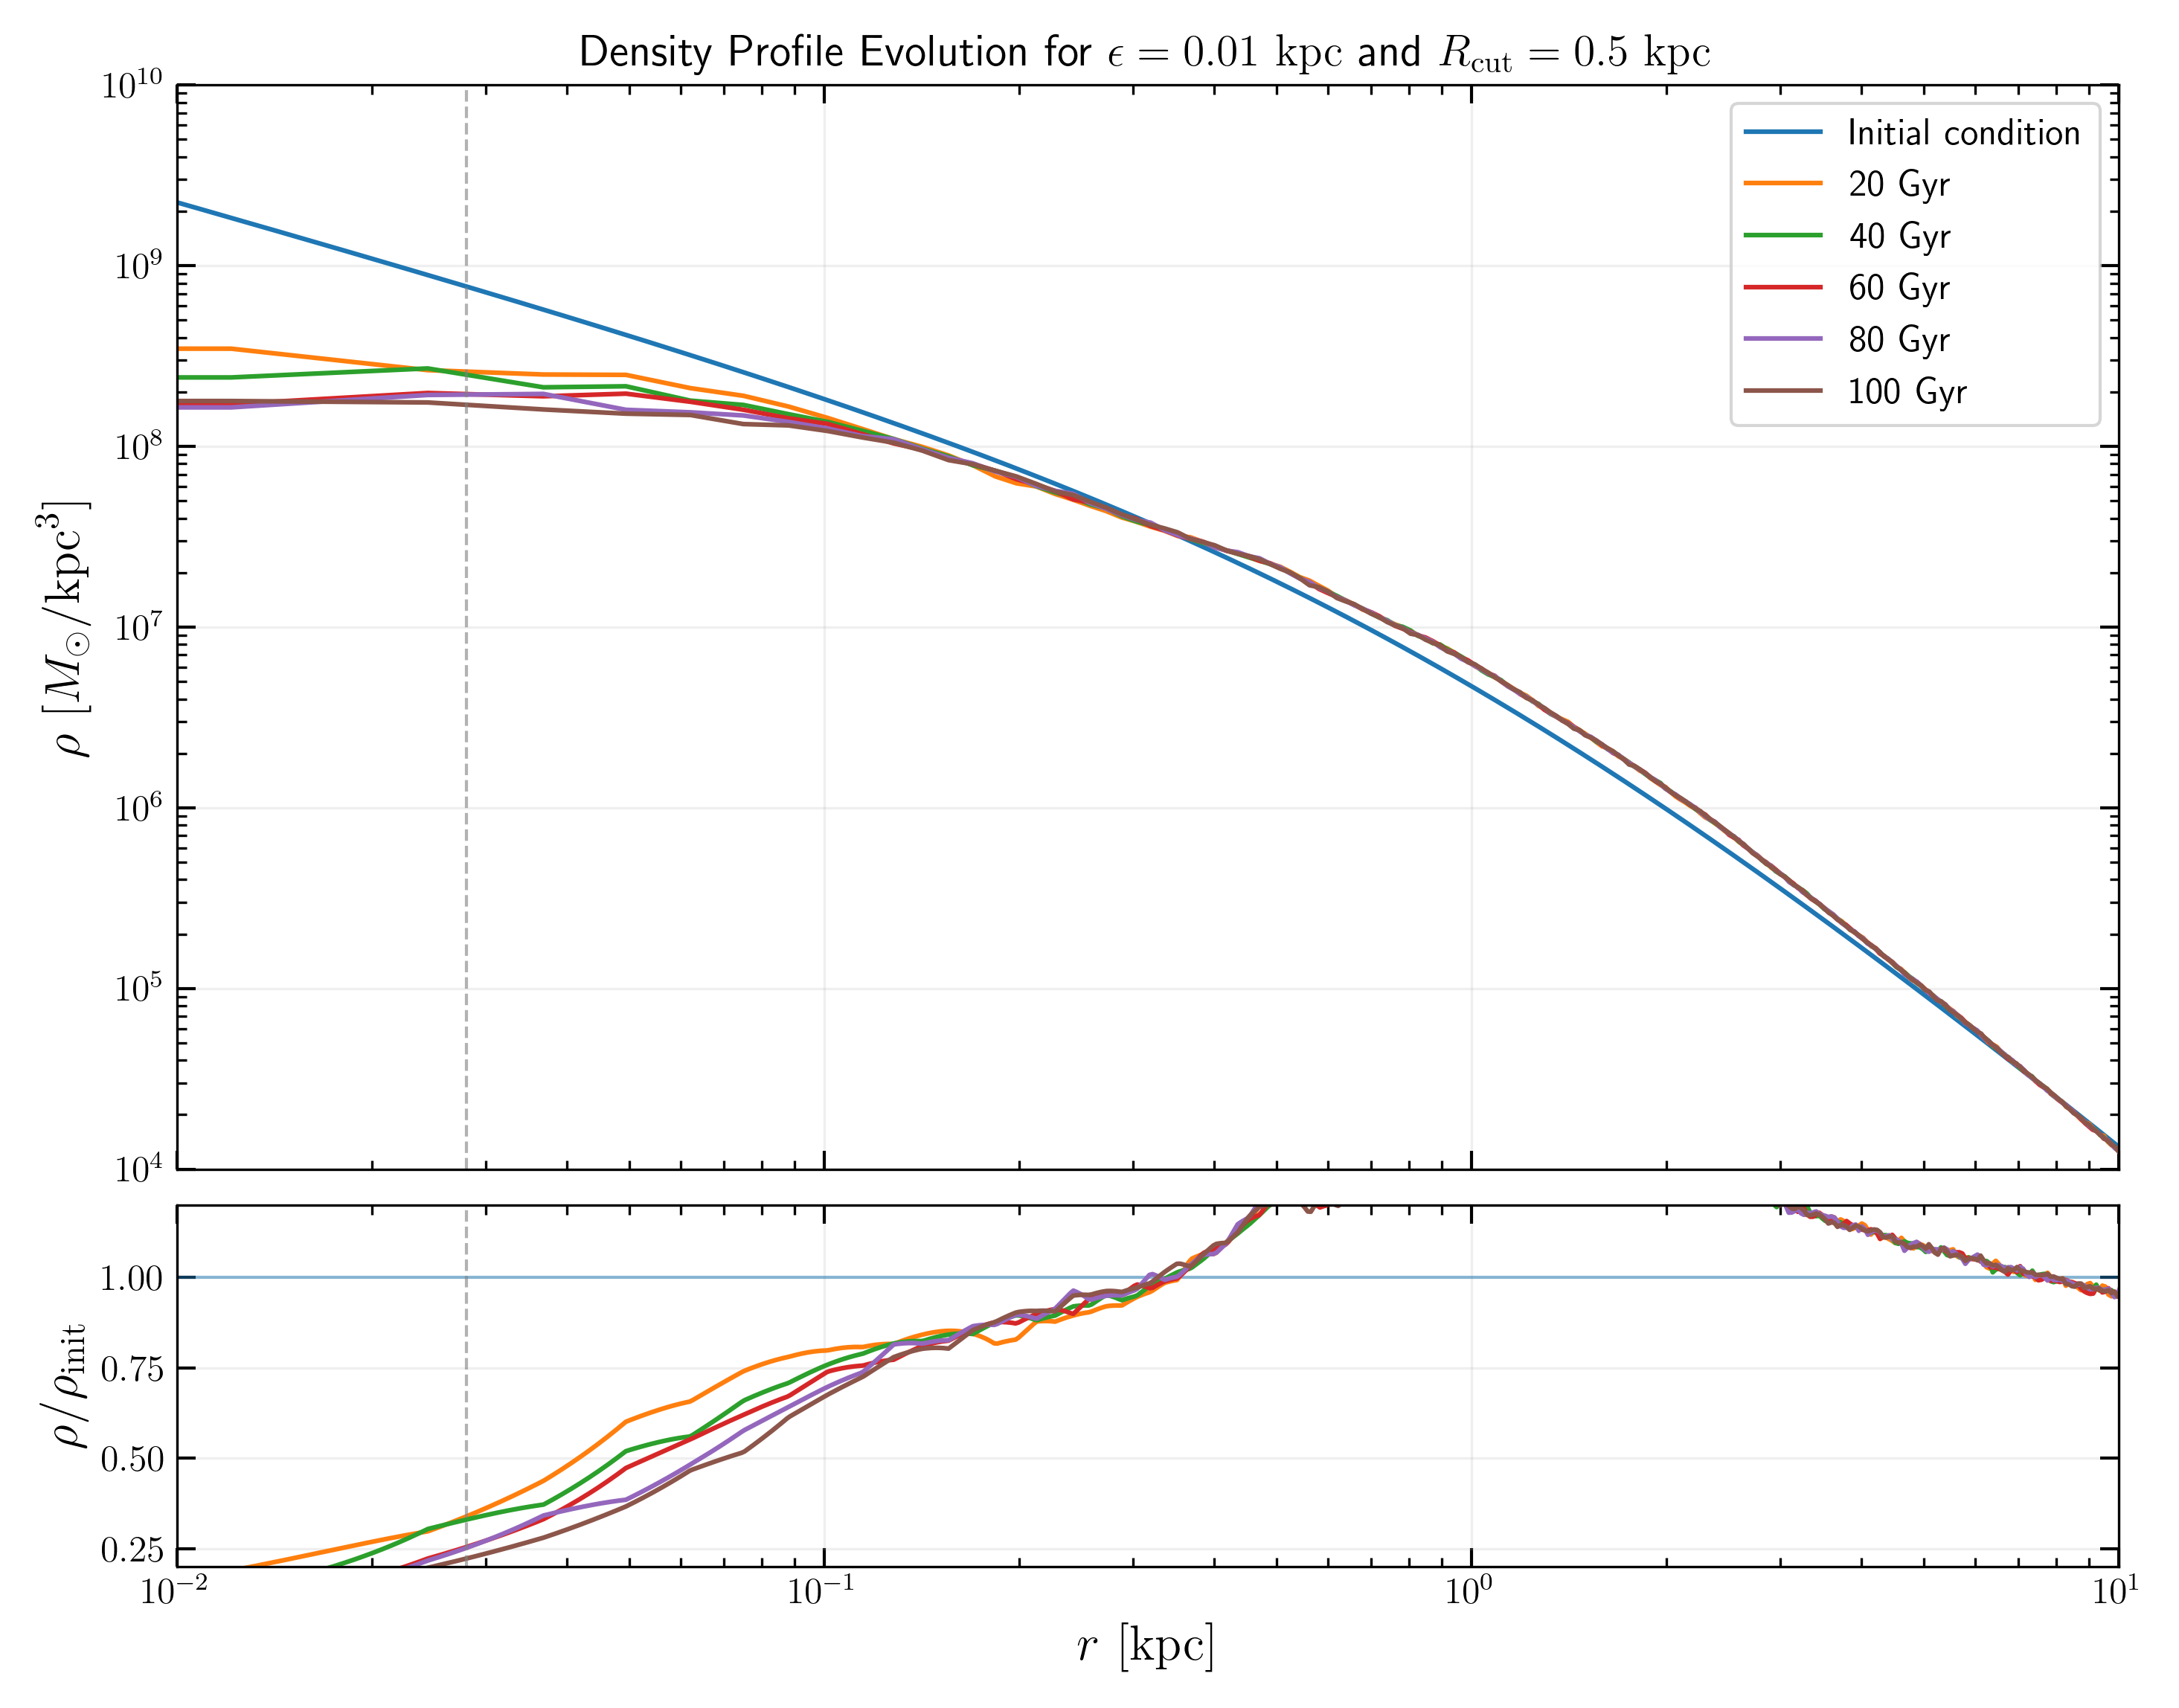
\includegraphics[width=0.9\textwidth]{0.5.png}
\end{figure}

\begin{figure}[H]
    \centering
    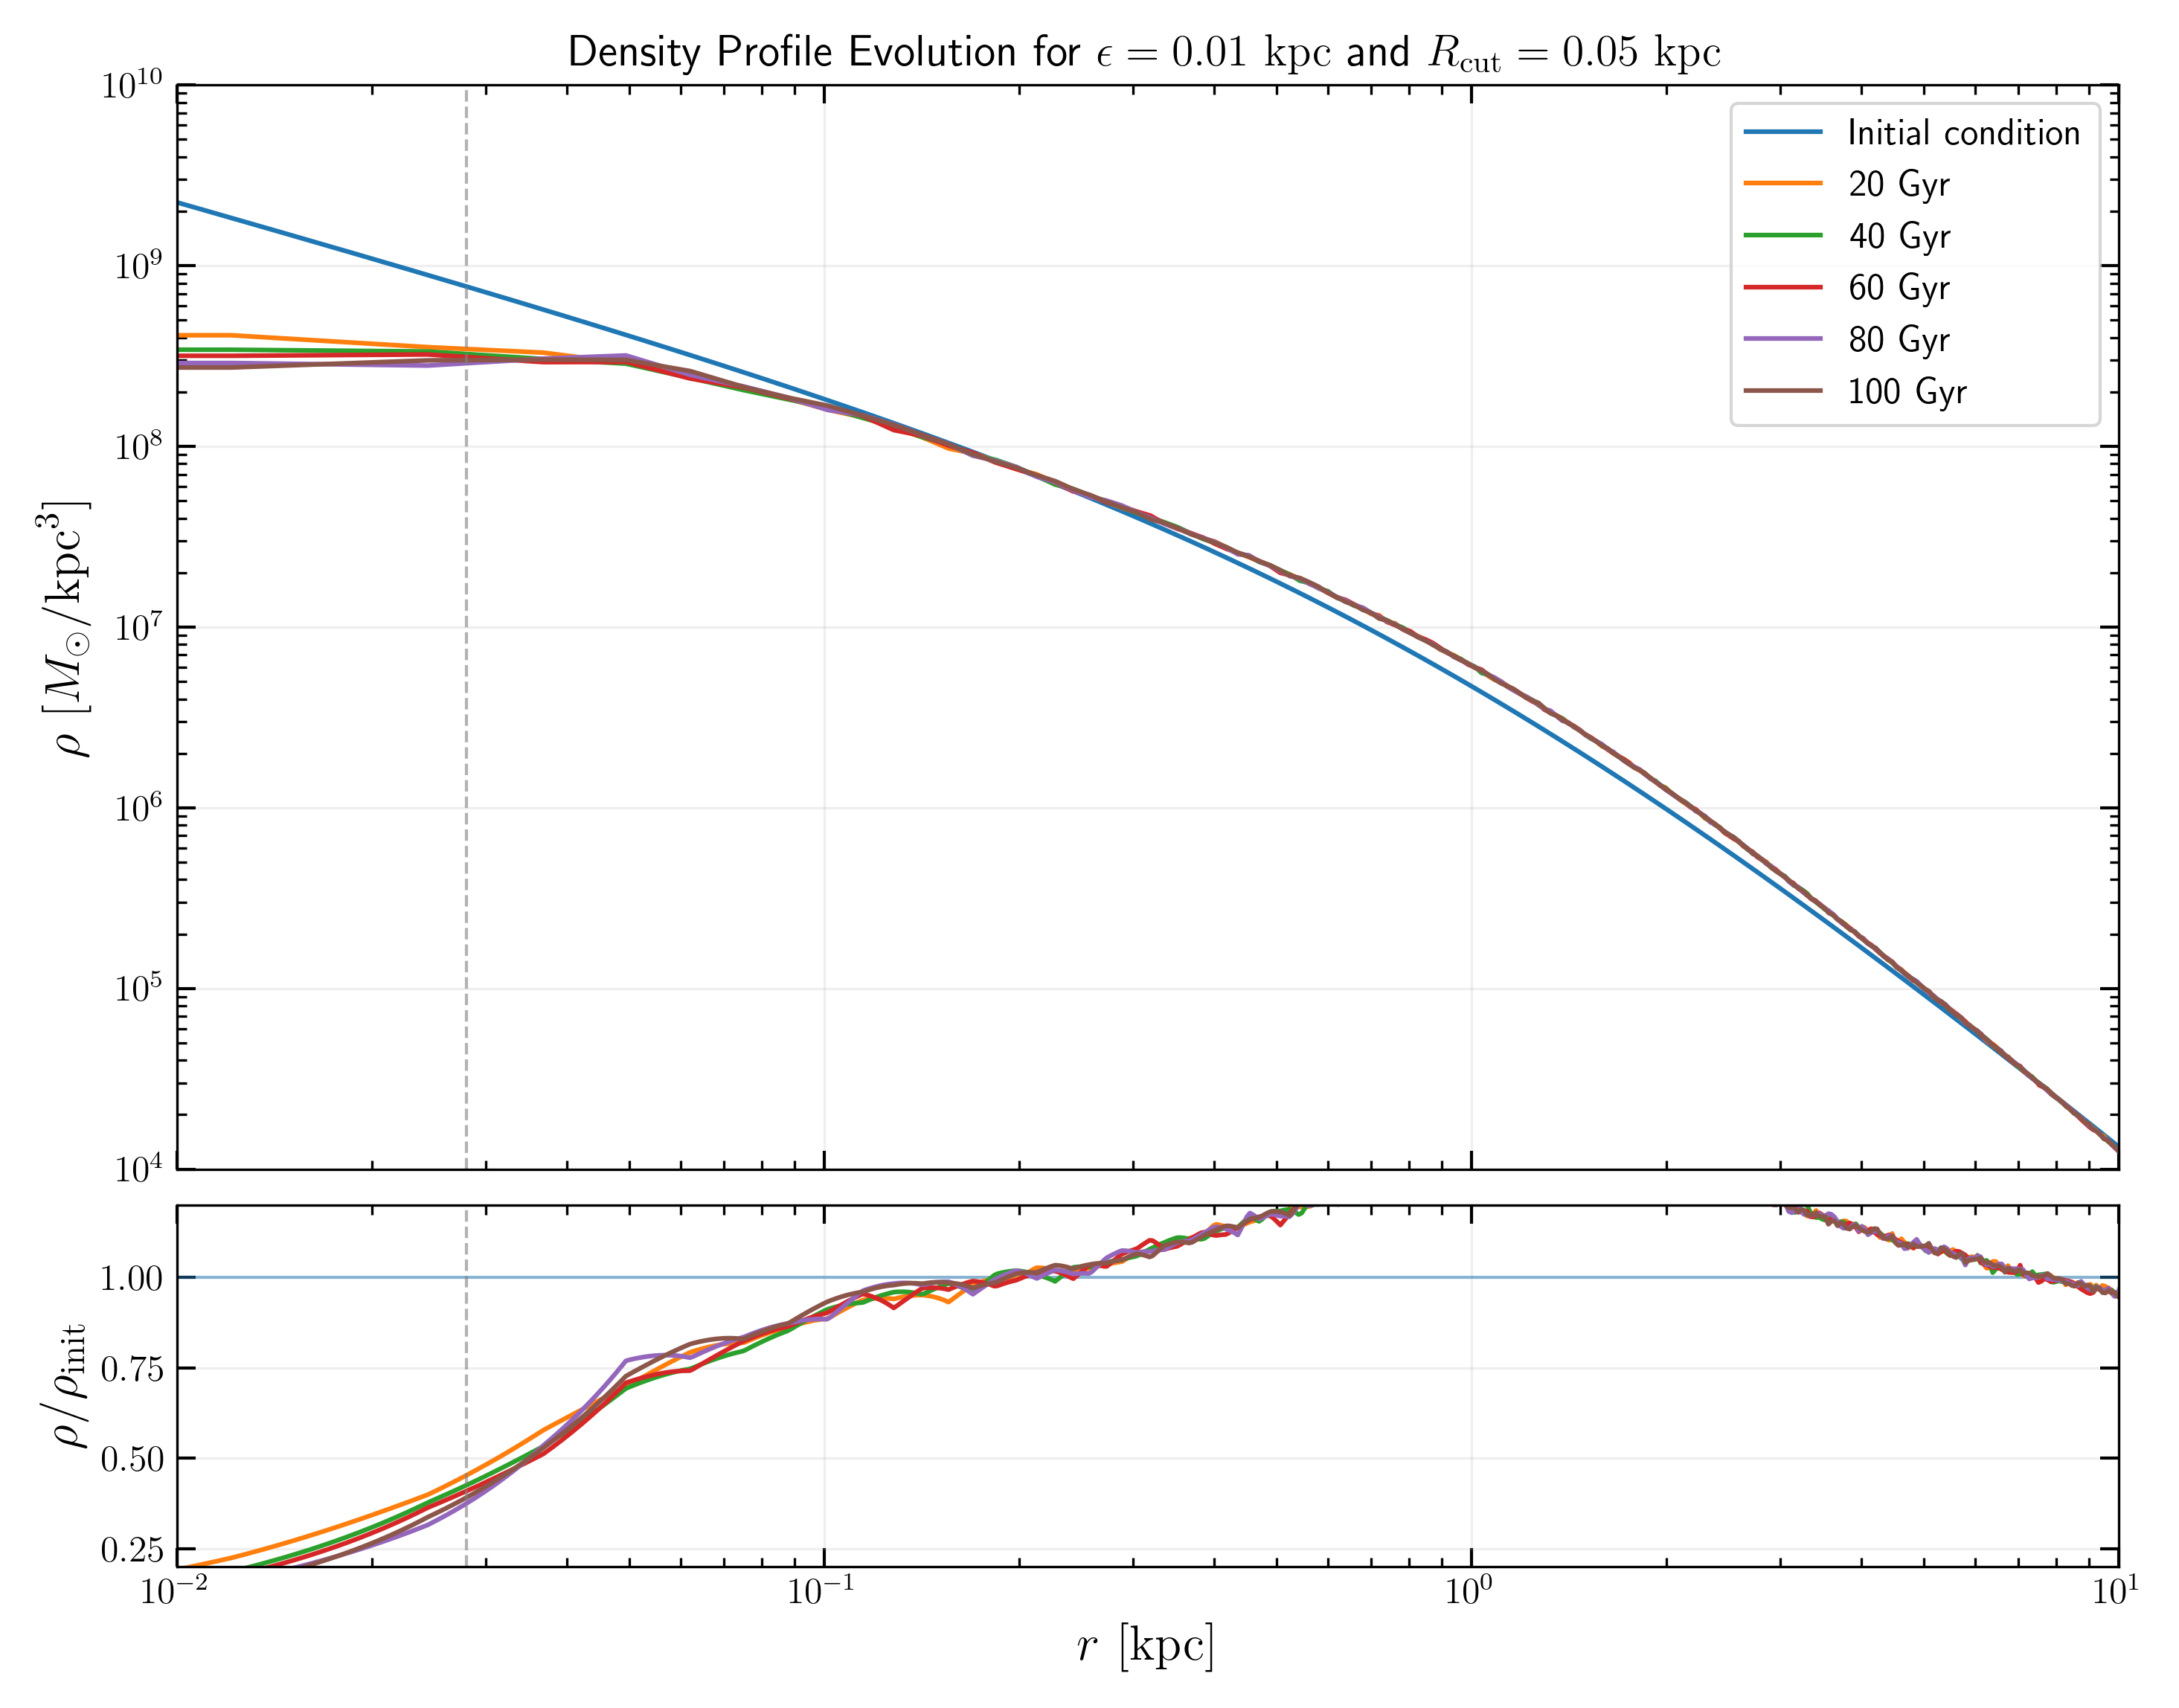
\includegraphics[width=0.9\textwidth]{0.05.png}
\end{figure}

\begin{figure}[H]
    \centering
    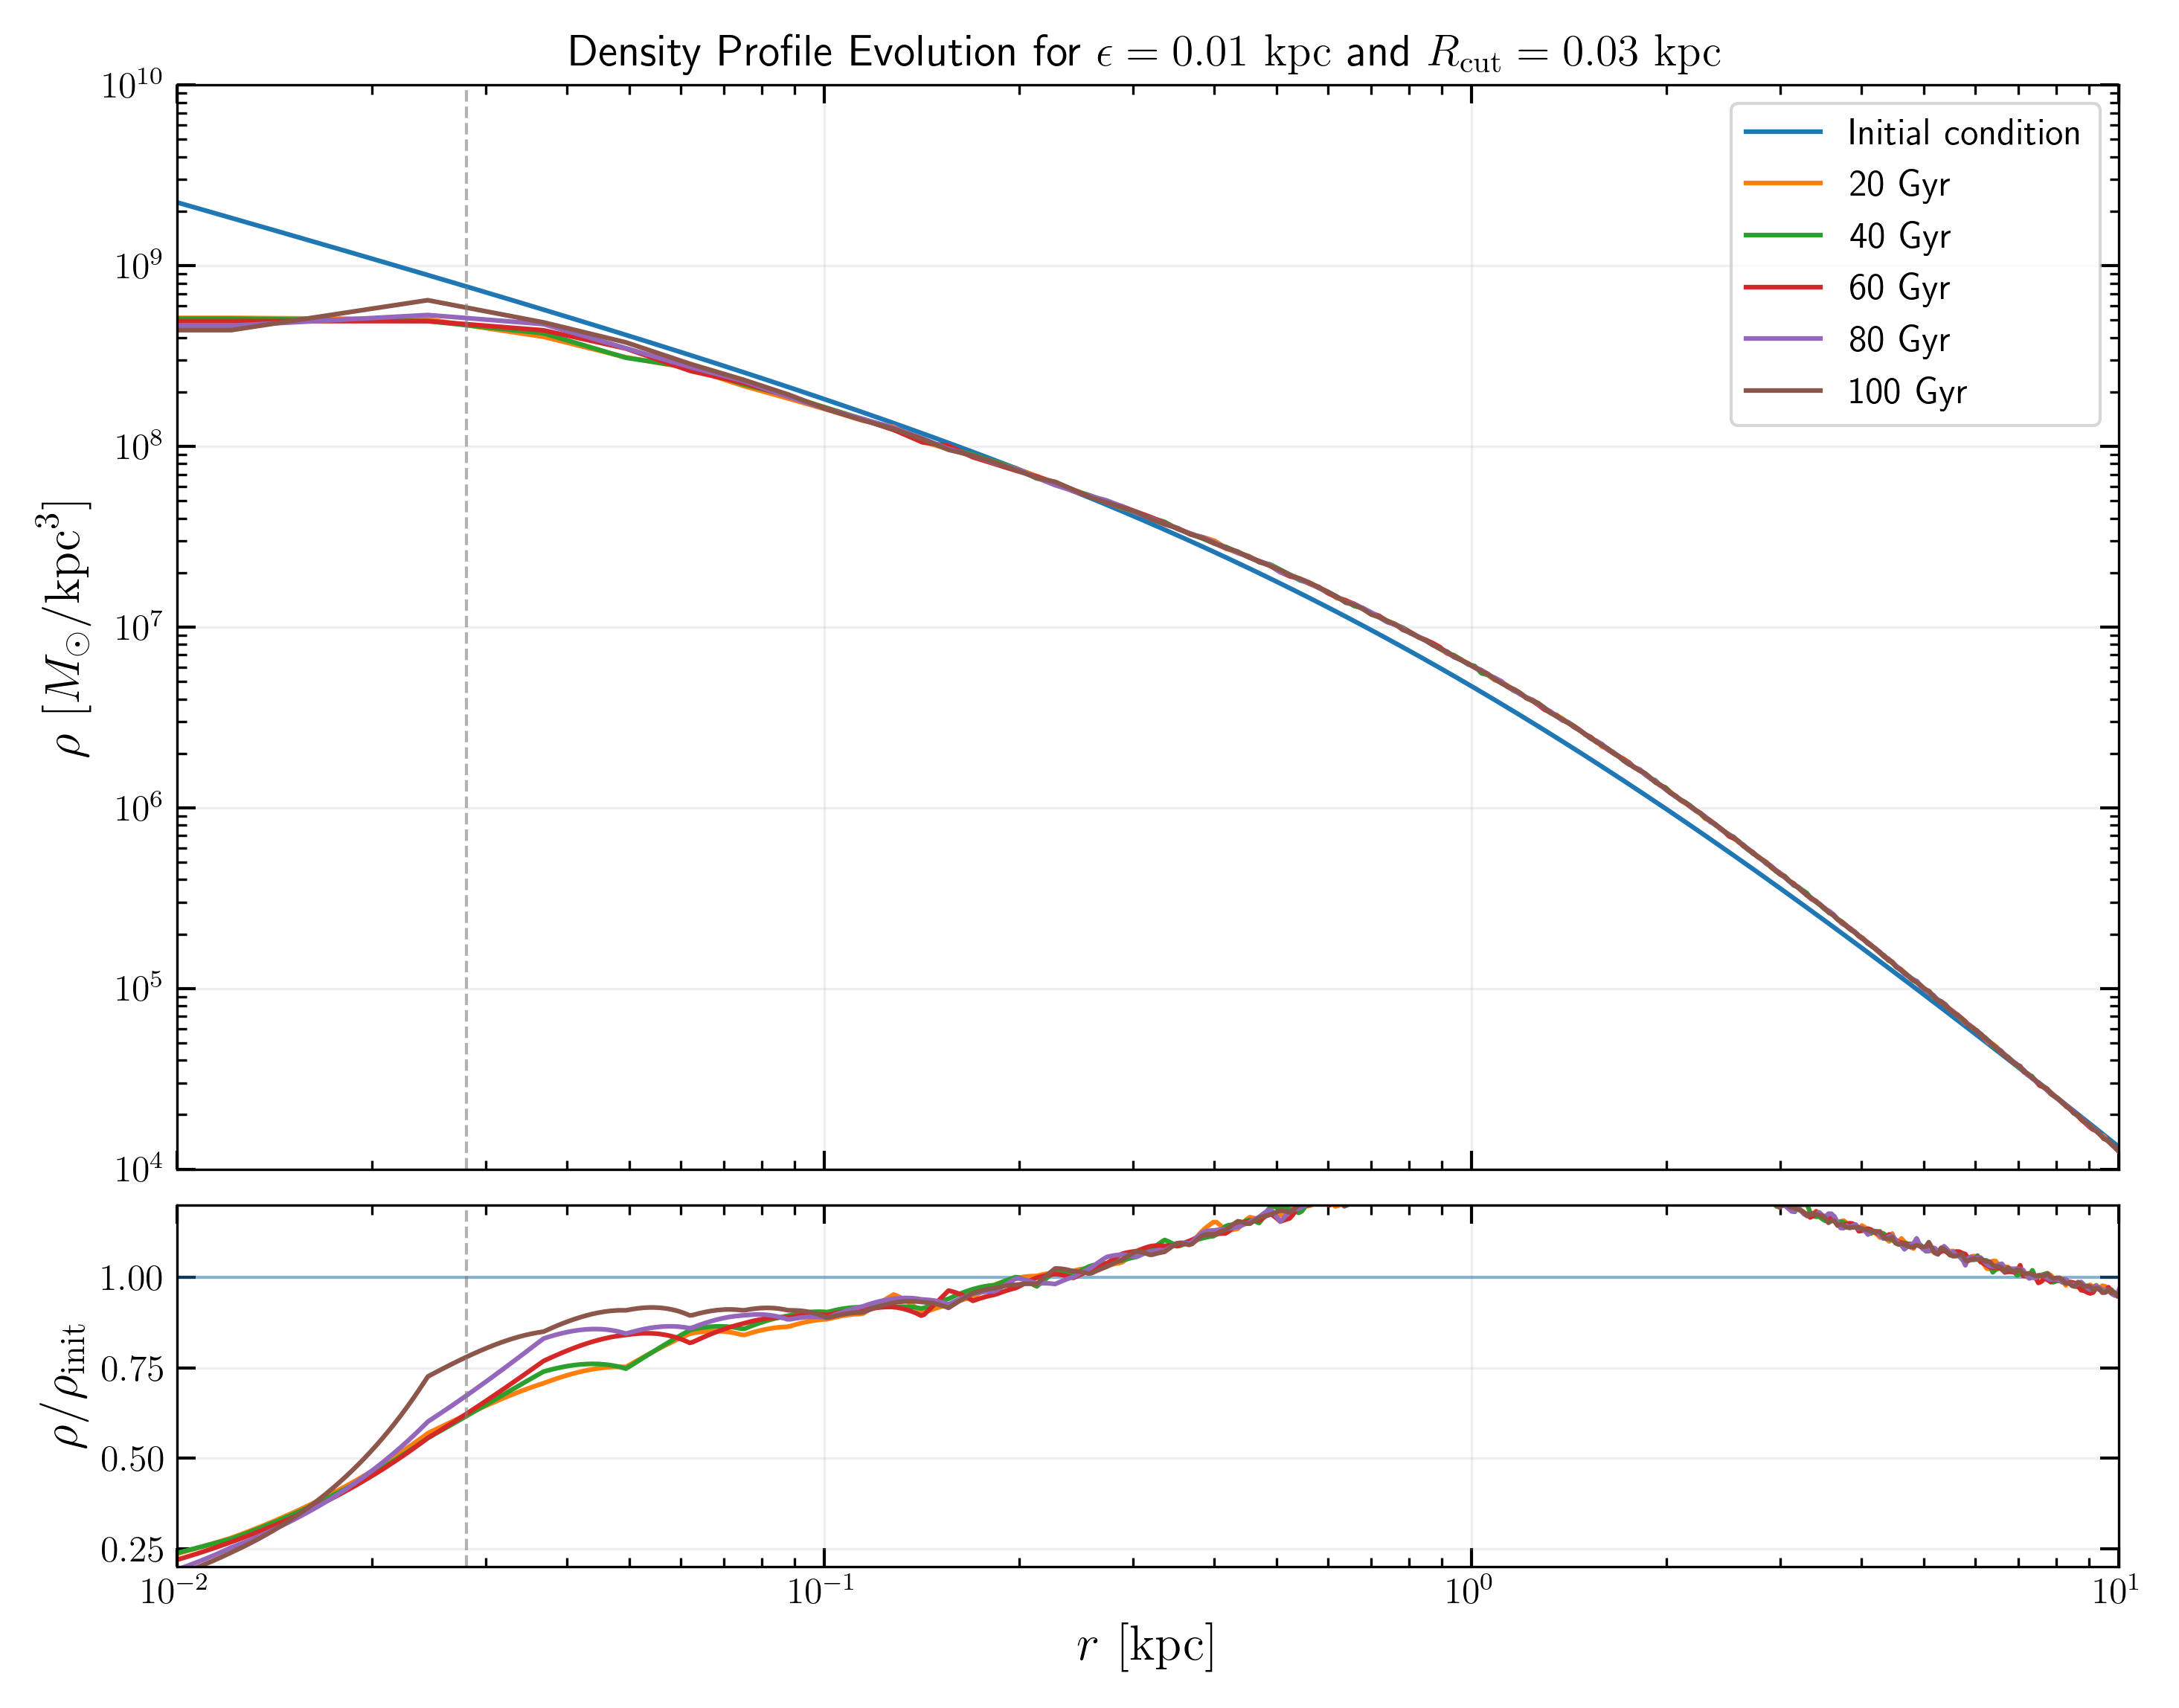
\includegraphics[width=0.9\textwidth]{0.03.png}
\end{figure}

\begin{figure}[H]
    \centering
    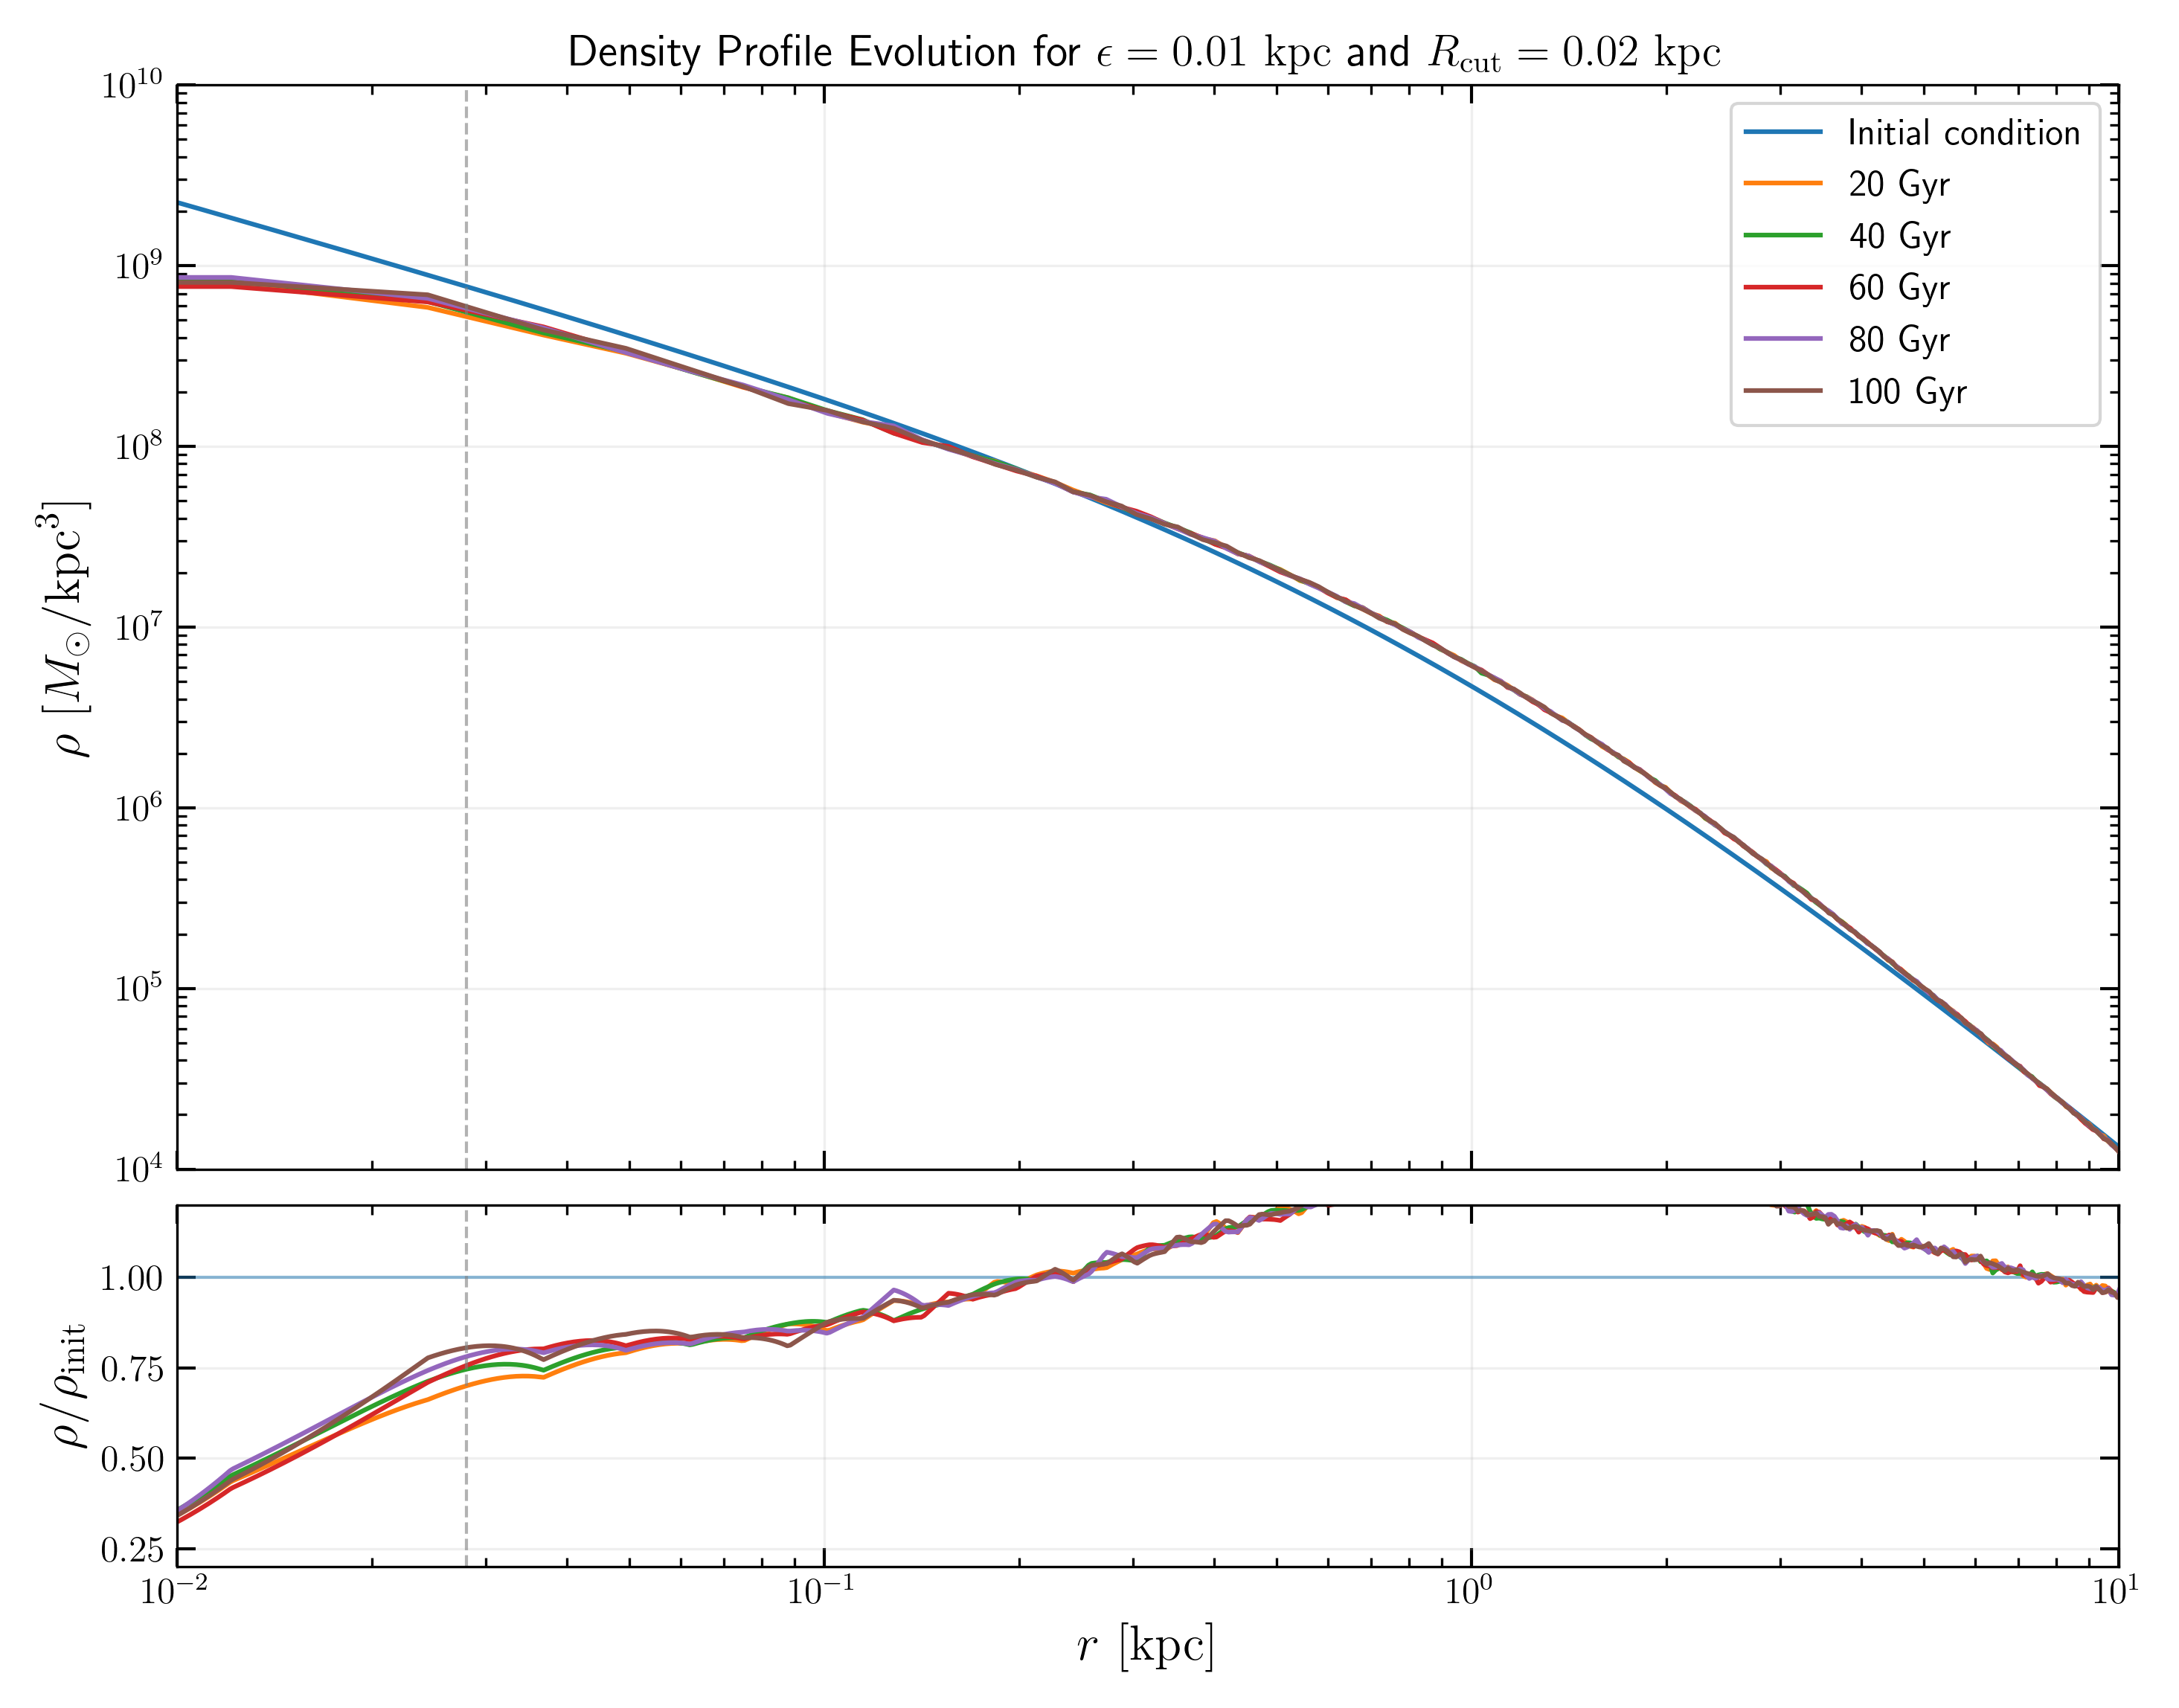
\includegraphics[width=0.9\textwidth]{0.02.png}
\end{figure}

\end{document}